%xelatex
%shell-escape для minted
\documentclass[a4paper, 12pt, oneside]{extarticle}
\input{$UNI/.templates/settings/preamble.tex}
\input{$UNI/.templates/settings/font_styles.tex}
\input{$UNI/.templates/settings/minted_settings.tex}
\addbibresource{~/Documents/uni/bibliography.bib}

\usepackage[explicit]{titlesec}
% \usepackage[svgnames]{xcolor}

\renewcommand\Variant{0.4*exp(–0.12*x)}
% \newcommand\Date{DAY.MONTH.\the\year}
\newcommand\Type{\Lab} % \Lab \Pract \RGR
\Work{num}
% \newcommand\Number{NUMBER}
\newcommand\Topic{Чисельне \\
визначення похідної та \\
інтеграла функції (№ 3)}

\usepackage[breakable]{tcolorbox}

\usepackage{blindtext}

\titleformat{\section}
[display]
{\color{black}\normalfont\bfseries}
{}
{0pt}
{\begin{tcolorbox}[arc=0mm, colback=blue!10!white, boxrule=0.2mm, beforeafter skip=0pt, boxsep=0mm]{ #1}\end{tcolorbox}}

\titleformat{\subsection}
[display]
{\color{black}\normalfont\bfseries}
{}
{0pt}
{\begin{tcolorbox}[arc=0mm, colback=blue!10!white, boxrule=0.2mm, beforeafter skip=0pt, boxsep=0mm]{ #1}\end{tcolorbox}}

\titlespacing*{\section}{0pt}{0ex}{-4ex}
\titlespacing*{\subsection}{0pt}{0ex}{-4ex}

\usepackage{multirow}
\usepackage{makecell}
\usepackage{tabularx}

% \setlength{\textfloatsep}{12pt}
\newcommand\tcobx[1]{
\begin{tcolorbox}[breakable, arc=0mm, colback=white, boxrule=0.2mm, beforeafter skip=0pt]
	#1
\end{tcolorbox}
}

\begin{document}
\Margins

\Margins
%\begin{wrapfigure}[3]{l}{.27\textwidth}
%\includegraphics[width=.28\textwidth]{$UNI/.templates/lpnu_logo.png}
%\end{wrapfigure}

%\noindent\textbf{Прізвище:} \Lname \\
%\noindent\textbf{Ім'я:} \Fname \\
%\noindent\textbf{Група:} \Group \\
%\noindent\textbf{Варіант:} \Variant \\
%\noindent\textbf{Дата захисту:} \Date \\
%\\
%\noindent\textbf{Кафедра:} \Department \\
%\noindent\textbf{Дисципліна:} \Discipline \\
%\noindent\textbf{Перевірив:} \Instructor \\

%%\medskip\bigskip

%\begin{center}
%	\textbf{ЗВІТ}		\\
%	до \Type~\No\Number	\\
%	на тему ``\Topic''	\\
%\end{center}

% \begin{table}
%   \begin{tabularx}{\textwidth}{|c|X|X|}
%     \hline
%     % Image & Content & Additional Info \\
%     % \hline
% 	  \multirow{3}{*}{\includegraphics[width=4cm]{$UNI/.templates/lpnu_logo.png}}
% 	  & \textbf{ЗВО:}
% 	  Національний університет ``Львівська Політехніка''.
% 	  & \textbf{Тема:}
% 	  \Topic
% 	  \\
% 	  & \textbf{Навчальний рік:}
% 	  2023/2024
% 	  & \textbf{Інститут}
% 	  комп'ютерних наук та інформаційних технологій
% 	  \\
% 	  & \textbf{Семестр:}
% 	  осінній
% 	  & \textbf{Група:}
% 	  \Group
% 	  \\
% 	  & \textbf{Навчальна дисципліна:}
% 	  \Discipline
% 	  & \textbf{Студент:}
% 	  Мілюхін Олександр
% 	  \\
% 	  & \textbf{Кафедра}
% 	  систем автоматизованого проектування
% 	  &
% 	  \\
% 	  & \textbf{Викладач:}
% 	  Чумакевич В. В.
% 	  &
% 	  \\
%     \hline
%   \end{tabularx}
% \end{table}

\setlength{\textfloatsep}{-16pt}
% \setlength{\intextsep}{0pt}

\begin{table}
	\begin{tabular}{|l|l|p{6cm}|}
    \hline
    % Image & Content & Additional Info \\
    % \hline
	  \makecell[l]{
	  \includegraphics[width=3.37cm]{$UNI/.templates/lpnu_logo.png}
  }
	  & \makecell[l]{
	  \textbf{ЗВО:}
	  Національний університет \\ ``Львівська Політехніка''.
	  \\
	  \textbf{Навчальний рік:}
	  2023/2024
	  \\
	  \textbf{Семестр:}
	  осінній
	  \\
	  \textbf{Навчальна дисципліна:} \\
	  \Discipline
	  \\
	  \textbf{Кафедра}
	  систем автоматизованого \\ проектування
	  \\
	  \textbf{Викладач:}
	  Чумакевич В. В.
}
	  & \makecell [l] {
	  \textbf{Тема:}
	  \Topic
	  \\
          \textbf{Інститут}
	  комп'ютерних наук та \\ інформаційних технологій
	  \\
	  \textbf{Група:}
	  \Group
	  \\
	  \textbf{Студент:}
	  Мілюхін Олександр
  }
  \\
    \hline
  \end{tabular}
\end{table}
\section{Мета роботи}

% \begin{table}
%   \begin{tabularx}{\textwidth}{|p{6cm}|c|c|}
% 	  \hline
%     \multirow{3}{*}{\includegraphics[width=6cm]{$UNI/.templates/lpnu_logo.png}}
% 	  & ЗВО: Національний університет ``Львівська Політехніка''
% 	  & Additional Info 1 \\
%     & Content 2 & Additional Info 2 \\
%     & Content 3 & Additional Info 3 \\
% 	  \hline
%   \end{tabularx}
% \end{table}

% \begin{table}
%   \begin{tabular}{|c|c|c|}
%     \hline
%     \multirow{3}{*}{\includegraphics[width=3cm]{$UNI/.templates/lpnu_logo.png}} & \makecell{Content 1 \\ Content 2 \\ Content 3} & \makecell{Additional Info 1 \\ Additional Info 2 \\ Additional Info 3} \\
%     \hline
%   \end{tabular}
% \end{table}

\tcobx{
Визначити для заданої функції похідну на основі різницевих виразів та інтеграл на основі формул
квадратури.
}

\section*{Індивідуальне завдання}
\tcobx{

1. Згідно із варіантом, одержати значення функції f(x).

2. Знайти аналітичний вираз

- похідної функції та обчислити його для x = 0

- первісної функції і обчислити його для меж від 0 до нескінченності.

3. Скласти програму, яка на основі різницевих формул

	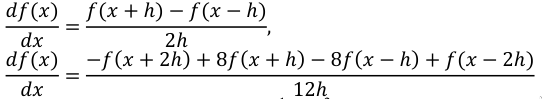
\includegraphics[width=.6\textwidth]{img/f1.png}

	визначає для кроків $h = \{1, 10^{–1}, 10^{–2} …\}$ похідну, а також, яка на основі формул складеної квадратури

	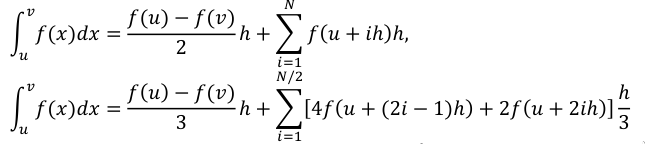
\includegraphics[width=.7\textwidth]{img/f2.png}

	обчислює для кількості інтервалів $N = {10, 10^2, …}$ визначений інтеграл.

4. Запустити програму на виконання та одержати результат через консоль.

5. Звести результатами обчислення у таблиці та побудувати графік відносної похибки обчислення
похідної залежно від вибраного кроку, а також графік відносної похибки обчислення визначеного
інтегралу залежно від вибраної кількості інтервалів.
}

\section*{Дані згідно з варіантом}

\tcobx{
	\Variant
}

\section*{ Аналітичні вирази }

\subsection*{ Похідна функції та її значення в заданій точці }

\tcobx{

$$
	\frac{df(x)}{dx} =
	% \left(0.4e^{–0.12x}\right)
\frac{2}{5}\cdot {e}^{-\frac{3\,x}{25}}\cdot \left(-\frac{3\,x}{25}\right)'_{x}
= -\frac{6\,{e}^{-\frac{3\,x}{25}}}{125}
$$

$$
	\frac{df(0)}{dx}
	= -\frac{6}{125}
	\approx -0.048
$$
}

\subsection*{ Первісна функції та її значення для заданих меж }

\tcobx {
$$
	\int{\frac{2}{5\,{e}^{\frac{3\,x}{25}}}}{\;\mathrm{d}x}
	=\frac{2}{5}\int{\frac{1}{\,{e}^{\frac{3\,x}{25}}}}{\;\mathrm{d}x}
	= -\frac{2}{5} \cdot \frac{25}{3\,{e}^{\frac{3\,x}{25}}}+C
	= -\frac{10}{3e^{\frac{3\,x}{25}}}+C
$$

$$
	\int_0^{\infty}{\frac{2}{5\,{e}^{\frac{3\,x}{25}}}}{\;\mathrm{d}x}
	= - \frac{10}{3e^{\frac{3\infty}{25}}}
	+ \frac{10}{3e^{\frac{0}{25}}}
	= - \frac{10}{3e^{\infty}}
	+ \frac{10}{3}
	\approx \frac{10}{3}
	\approx 3.33333333333
$$
}

\section*{ Код програми}

\tcobx {
	\inputminted{c}{dergral.c}
}

\section*{ Вивід}

\tcobx {
% \verbatiminput{plot.csv}
	\verbatiminput{out}
}

\section*{ Результати обчислення}

\subsection*{ Таблиця з результатами обчислення похідної}

\tcobx {
\csvautolongtable{deriv.csv}
}

\subsection*{ Таблиця з результатами обчислення інтеграла}

\tcobx {
\csvautolongtable{int.csv}
}

\subsection*{ Графік відносної похибки обчислення похідної}

\tcobx {
\includegraphics{deriv.pdf}
}

\subsection*{ Графік відносної похибки обчислення інтеграла}

\tcobx {
\includegraphics{int.pdf}
}

\section*{ Висновок}

\tcobx {
Я обчислив похідну й інтеграл заданої функції аналітично,
після чого склав програму для їх наближеного обчислення
мовою С.З отриманих значень побудував
таблицю та графік за допомогою `gnuplot`.

Оптимальні кроки диференціювання:
\begin{itemize}
	\item для різницевої формули 2-го порядку: \texttt{h = 1.00e-05}
	\item для різницевої формули 4-го порядку: \texttt{h = 1.00e-02}
\end{itemize}
}

\end{document}
